%%%%%%%%%%%%%%%%%%%%%%%%%%%%%%%%%%%%%%%%%
% University/School Laboratory Report
% LaTeX Template
% Version 3.1 (25/3/14)
%
% This template has been downloaded from:
% http://www.LaTeXTemplates.com
%
% Original author:
% Linux and Unix Users Group at Virginia Tech Wiki 
% (https://vtluug.org/wiki/Example_LaTeX_chem_lab_report)
%
% License:
% CC BY-NC-SA 3.0 (http://creativecommons.org/licenses/by-nc-sa/3.0/)
%
%%%%%%%%%%%%%%%%%%%%%%%%%%%%%%%%%%%%%%%%%

%----------------------------------------------------------------------------------------
%	PACKAGES AND DOCUMENT CONFIGURATIONS
%----------------------------------------------------------------------------------------

\documentclass{article}

\usepackage[version=3]{mhchem} % Package for chemical equation typesetting
\usepackage{siunitx} % Provides the \SI{}{} and \si{} command for typesetting SI units
\usepackage{graphicx} % Required for the inclusion of images
\usepackage{natbib} % Required to change bibliography style to APA
\usepackage{amsmath} % Required for some math elements 
\usepackage[utf8]{inputenc}
\usepackage{tikz,pgfplots}
\usepackage[letterpaper, margin=0.2in]{geometry}
\usepackage{float}
\usepackage{enumitem}
\usepackage{fixltx2e}
\usepackage{gensymb}
\usepackage[hidelinks]{hyperref}
\usepackage[all]{hypcap}

\usepackage{xcolor}

% Roman numerials
\pagenumbering{arabic}

\setlength\parindent{0pt} % Removes all indentation from paragraphs

%\renewcommand{\labelenumi}{\alph{enumi}.} % Make numbering in the enumerate environment by letter rather than number (e.g. section 6)

%\usepackage{times} % Uncomment to use the Times New Roman font

% for some tables
\newcommand{\specialcell}[2][c]{%
  \begin{tabular}[#1]{@{}c@{}}#2\end{tabular}}
  
\providecommand{\e}[1]{\ensuremath{\times 10^{#1}}}
%----------------------------------------------------------------------------------------
%	DOCUMENT INFORMATION
%----------------------------------------------------------------------------------------

%\title{Determination of the Atomic \\ Weight of Magnesium \\ CHEM 101} % Title

%\author{John \textsc{Smith}} % Author name

%\date{\today} % Date for the report

\begin{document}

%\maketitle % Insert the title, author and date

% If you wish to include an abstract, uncomment the lines below
% \begin{abstract}
% Abstract text
% \end{abstract}

%----------------------------------------------------------------------------------------
%	SECTION 1
%----------------------------------------------------------------------------------------


\section{Arch Appliance Stuff}

\Large{Plots of AA time retrieval. I messed up the matlab titles and did not want to recombile (takes a long time). Left one is only non-bergoz BPMs with 43 PVs. Right side is Bergoz BPMs with 77 PVs. Note that the first data point(~\#200) on the right side takes more time than the last data point(~\#18000) on the left side!}


\begin{figure}[H]
\centering
\begin{tikzpicture}
\node at (0,0) {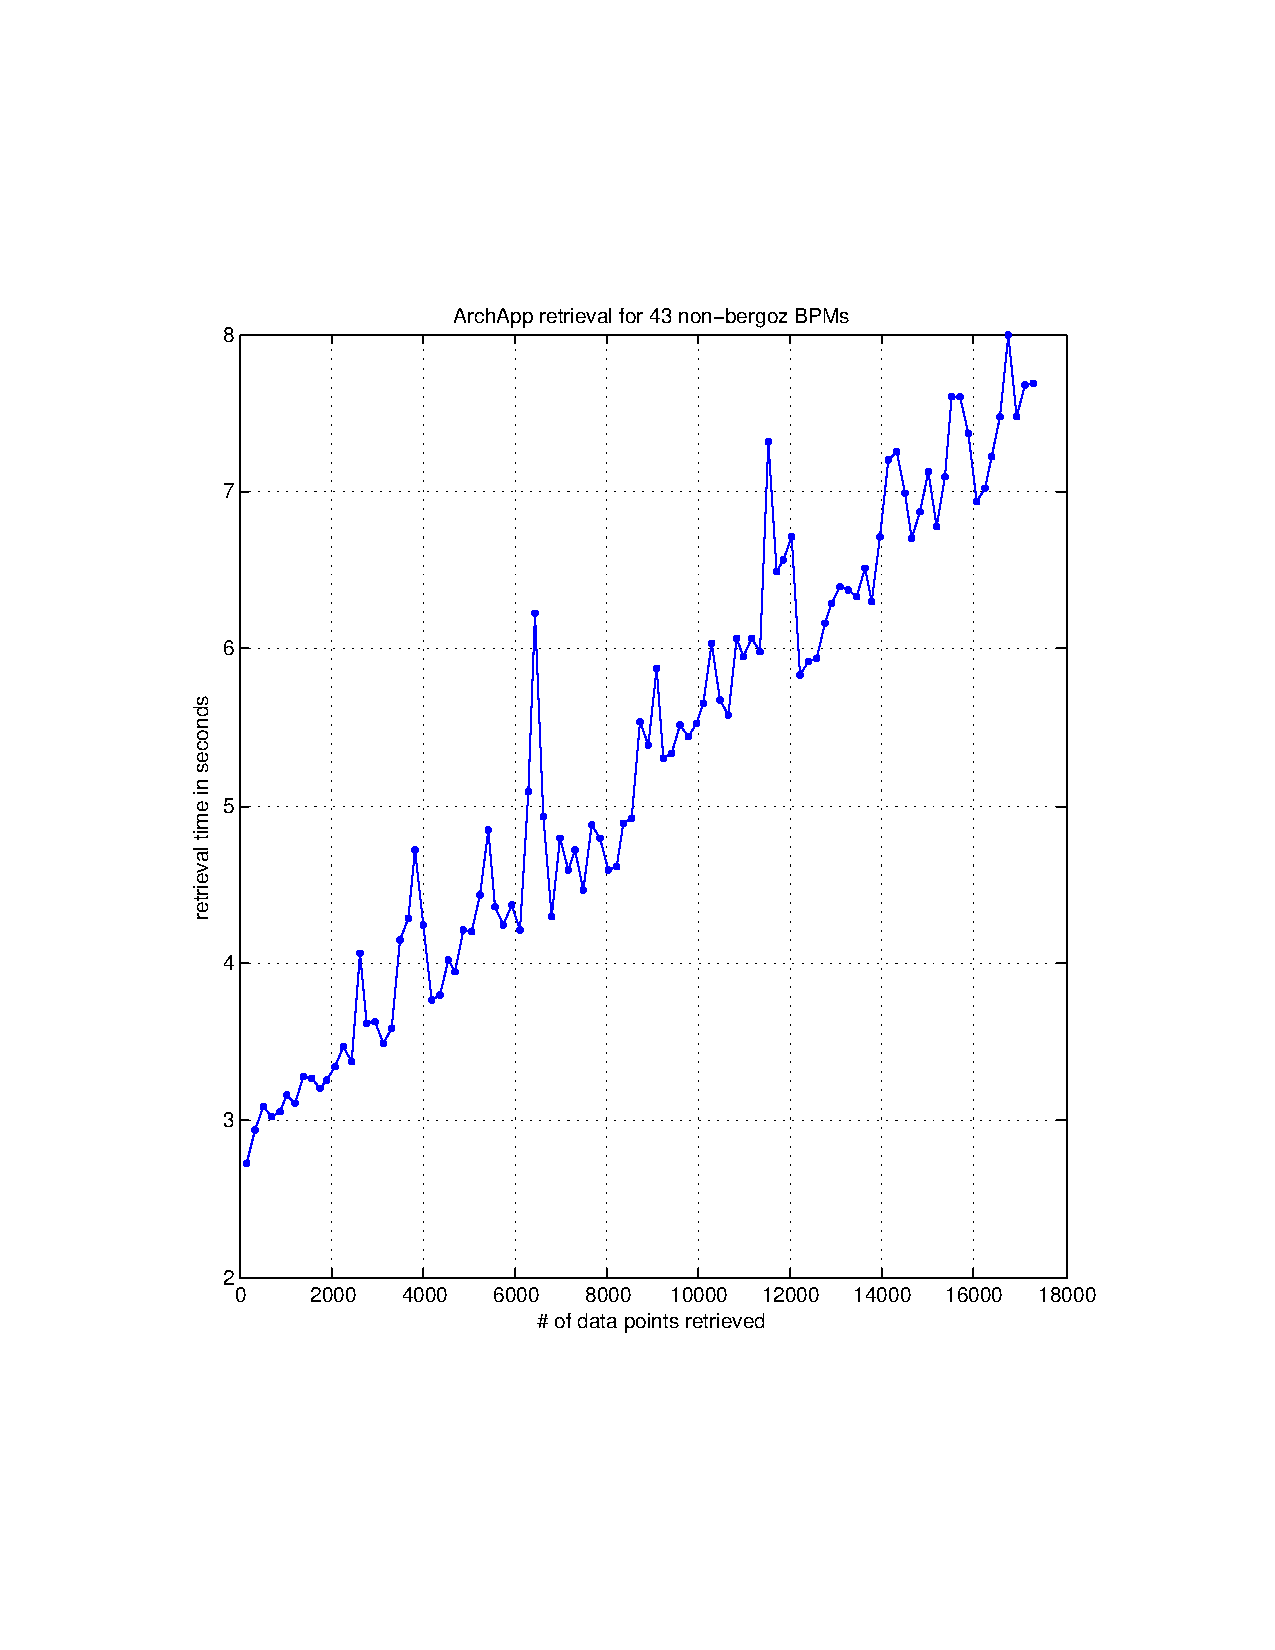
\includegraphics[height=400pt]{nonbergoz_43BPMs.pdf}};
\node at (10,0) {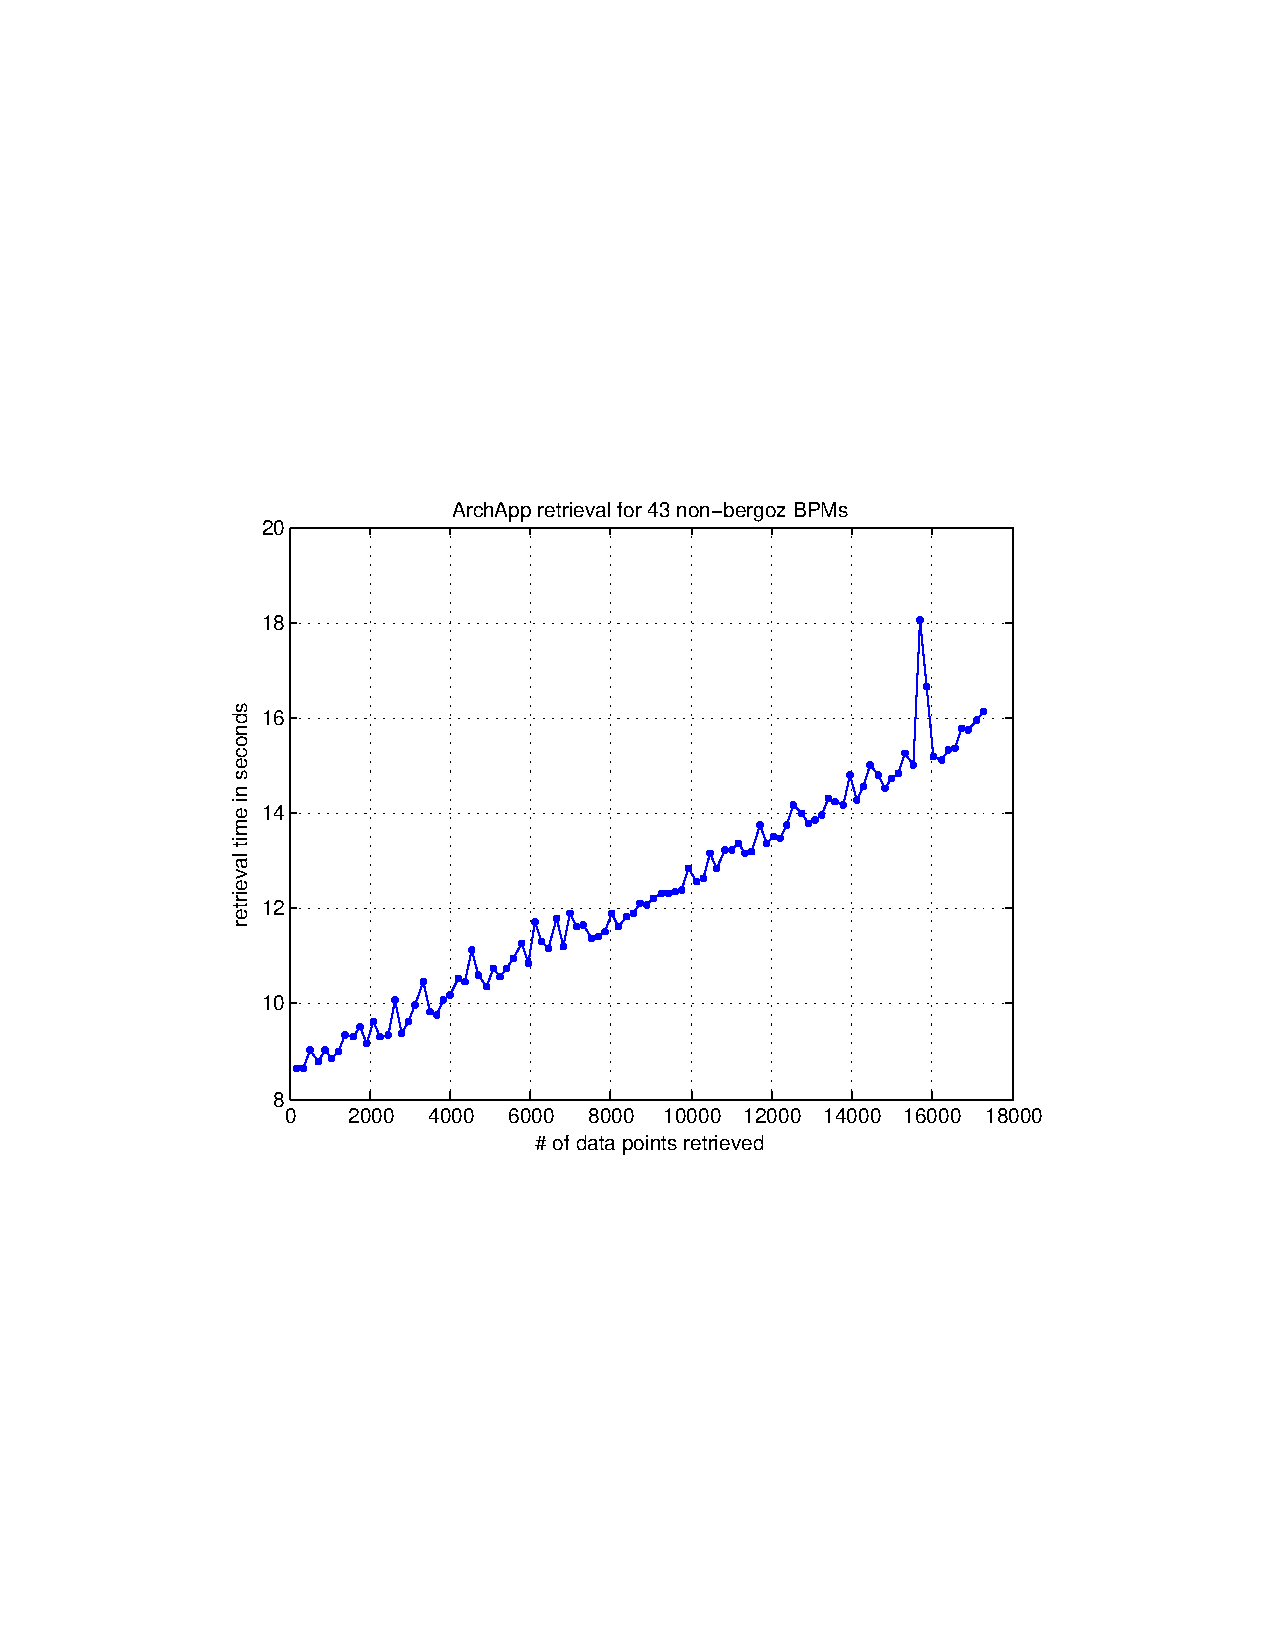
\includegraphics[height=500pt]{bergoz_77BPMs.pdf}};
\draw[-] (-1.7,4.35) -- (1.7,4.35);
\node at (0,4.8) {\large{AA retrieval for non-bergoz BPMs (43 PVs).}};
\draw[-] (8,3.35) -- (12.3,3.35);
\node at (11,3.9) {\large{AA retrieval for bergoz BPMs (77 PVs).}};
\end{tikzpicture}
\end{figure}

l\\*[5cm]

Here is a screen shot comparison of the data (the gui would not let me save a high res copy). Left side is using AA and right side is using the ChannelArchiver. Note the slightly off values here; it is most obvious in the beginning of the last plot. Also ignore the last 1 hour of data as that is caused by the off by 1 hour AA stuff.

\begin{figure}[H]
\centering
\begin{tikzpicture}
\node at (0,0) {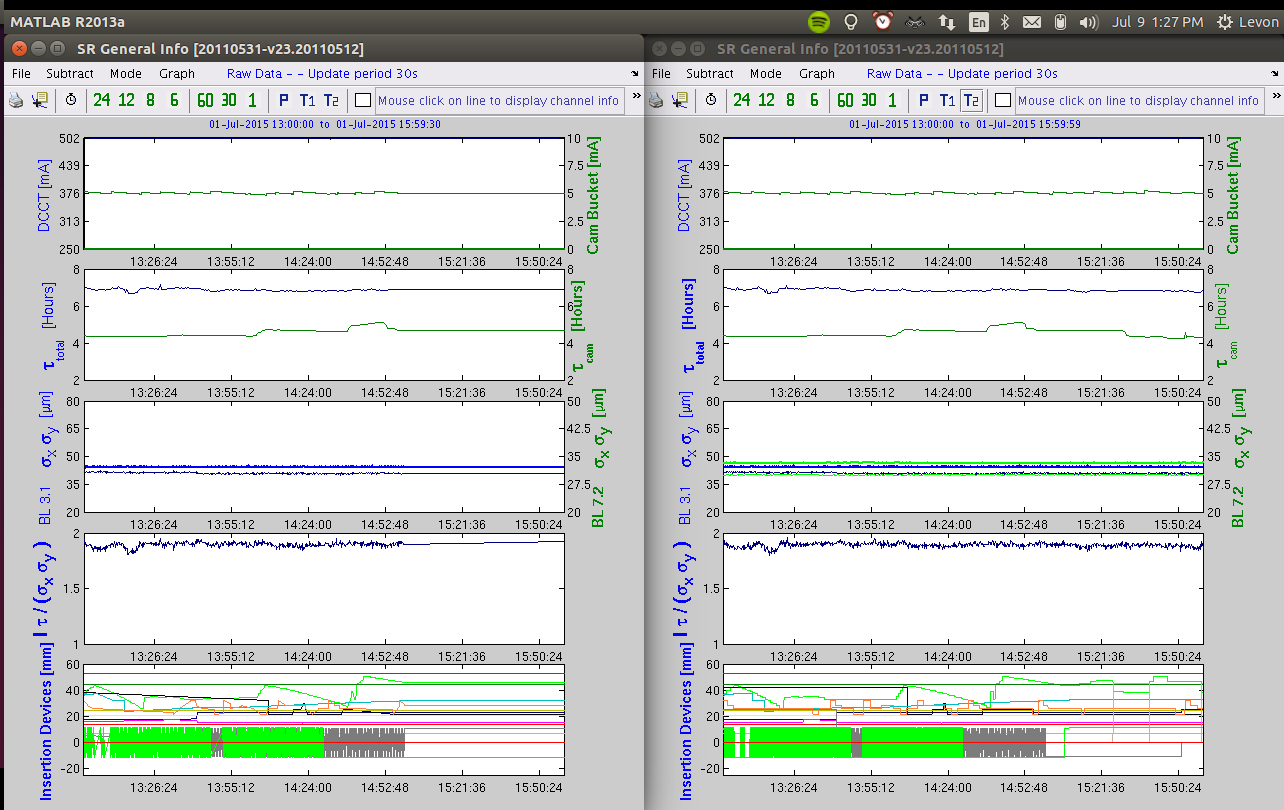
\includegraphics[width=500pt]{scrnshot.png}};

\end{tikzpicture}
\end{figure}



%	SECTION 5
%----------------------------------------------------------------------------------------


%----------------------------------------------------------------------------------------
%	SECTION 6
%----------------------------------------------------------------------------------------

% Nothing right now

%----------------------------------------------------------------------------------------
%	BIBLIOGRAPHY
%----------------------------------------------------------------------------------------

\bibliographystyle{apalike}

\bibliography{sample}

%----------------------------------------------------------------------------------------


\end{document}













